\documentclass[border=6pt]{standalone}
\usepackage{tikz}
\usetikzlibrary{arrows.meta,positioning,calc,shapes.geometric,fit,backgrounds,patterns,matrix,decorations.pathreplacing}
\begin{document}
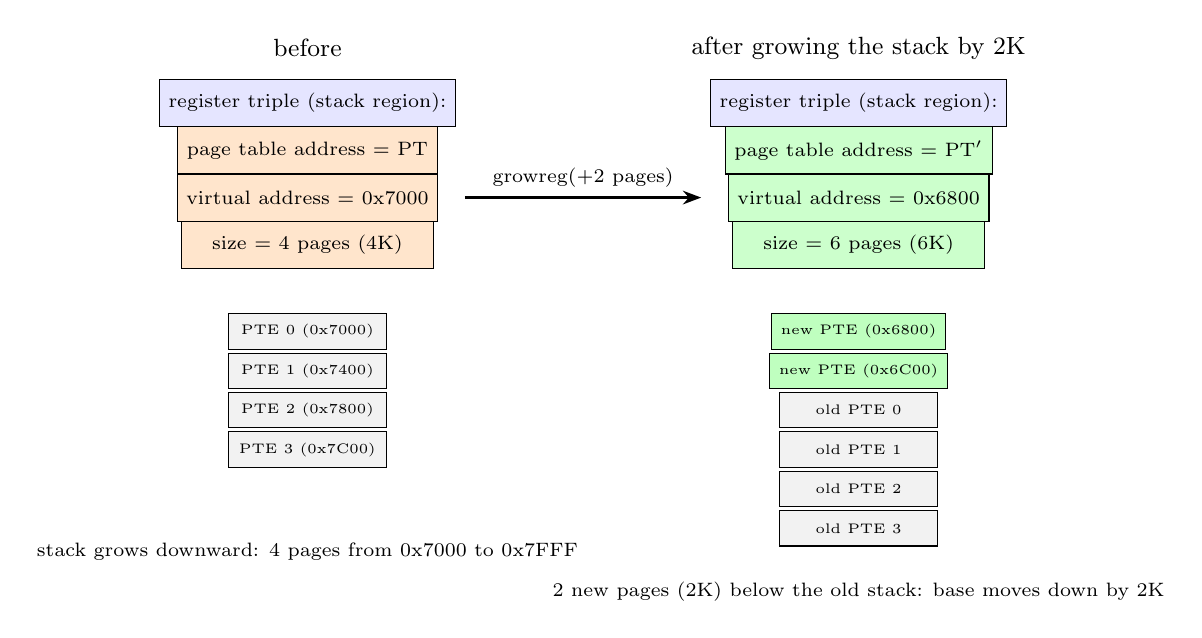
\begin{tikzpicture}[>=Stealth,font=\small]
\tikzstyle{c}=[draw,minimum height=0.6cm,minimum width=3.2cm,font=\scriptsize,align=center]
\node[font=\small] at (2,2.2) {before};
\node[c,fill=blue!10] at (2,1.5) {register triple (stack region):};
\node[c,fill=orange!20] at (2,0.9) {page table address = PT};
\node[c,fill=orange!20] at (2,0.3) {virtual address = 0x7000};
\node[c,fill=orange!20] at (2,-0.3) {size = 4 pages (4K)};
\node[font=\small] at (9,2.2) {after growing the stack by 2K};
\node[c,fill=blue!10] at (9,1.5) {register triple (stack region):};
\node[c,fill=green!20] at (9,0.9) {page table address = PT$'$};
\node[c,fill=green!20] at (9,0.3) {virtual address = 0x6800};
\node[c,fill=green!20] at (9,-0.3) {size = 6 pages (6K)};
\draw[->,thick] (4,0.3) -- (7,0.3) node[midway,above,font=\scriptsize]{growreg(+2 pages)};
\foreach \i/\y/\a in {0/-1.4/7000,1/-1.9/7400,2/-2.4/7800,3/-2.9/7C00} \node[draw,minimum width=2cm,minimum height=0.45cm,font=\tiny,fill=gray!10] at (2,\y) {PTE \i\ (0x\a)};
\foreach \i/\y in {-2/-1.4,-1/-1.9} \node[draw,minimum width=2cm,minimum height=0.45cm,font=\tiny,fill=green!25] at (9,\y) {new PTE (0x6\ifnum\i=-2 8\else C\fi00)};
\foreach \i/\y in {0/-2.4,1/-2.9,2/-3.4,3/-3.9} \node[draw,minimum width=2cm,minimum height=0.45cm,font=\tiny,fill=gray!10] at (9,\y) {old PTE \i};
\node[font=\scriptsize,align=left] at (2,-4.2) {stack grows downward: 4 pages from 0x7000 to 0x7FFF};
\node[font=\scriptsize,align=left] at (9,-4.7) {2 new pages (2K) below the old stack: base moves down by 2K};
\end{tikzpicture}
\end{document}
